\documentclass[a4paper]{article}
\usepackage[a4paper,margin=0mm]{geometry}
\usepackage{fontspec}
\usepackage{unicode-math}
\usepackage{tikz}
\usetikzlibrary{fit,calc,positioning,arrows.meta}
\usepackage[table]{xcolor}
\usepackage[absolute]{textpos}
\usepackage{array}

\setmainfont{Libertinus Serif}
\setsansfont{Libertinus Sans}
\setmathfont{Libertinus Math}

\definecolor{accent}{HTML}{602785}
\definecolor{badge}{HTML}{B8A0C8}
\definecolor{ink}{HTML}{2A2E30}

\setlength{\TPHorizModule}{1mm}
\setlength{\TPVertModule}{1mm}
\setlength{\parindent}{0pt}
\pagestyle{empty}

\newcommand{\topicheader}[2]{%
\begin{textblock*}{194mm}(16mm,10mm)
\begin{tikzpicture}
\node[fill=accent,text=white,font=\sffamily\bfseries\fontsize{13}{13}\selectfont,
      minimum width=9mm,minimum height=9mm,inner sep=0pt] at (4.5mm,-4.5mm) {#1};
\node[font=\sffamily\bfseries\fontsize{15}{16}\selectfont,text=ink,anchor=west] at (12mm,-4.5mm) {#2};
\end{tikzpicture}
\end{textblock*}
\begin{textblock*}{194mm}(16mm,22.5mm)

\begin{tikzpicture}
\fill[accent] (0,0) rectangle (194mm,0.5mm);
\end{tikzpicture}
\end{textblock*}
}

\newcommand{\pagekicker}[1]{%
\begin{textblock*}{100mm}(16mm,25.5mm)
\begin{tikzpicture}
\node[fill=ink,text=white,font=\sffamily\bfseries\fontsize{8}{8}\selectfont,
      inner sep=2.2pt,rounded corners=1pt] {\MakeUppercase{#1}};
\end{tikzpicture}
\end{textblock*}
}

\newcommand{\videobanner}[1]{%
\begin{textblock*}{178mm}(16mm,25.5mm)
\begin{tikzpicture}
\fill[accent] (0,0) rectangle (178mm,-10mm);
\draw[white,line width=0.6pt] (3mm,-1.7mm) rectangle (11.5mm,-8.3mm);
\node[white,font=\sffamily\fontsize{4}{4.4}\selectfont,align=center] at (7.25mm,-5mm) {QR\\CODE};
\node[white,font=\sffamily\bfseries\fontsize{9.5}{11}\selectfont,anchor=west] at (16mm,-5.6mm) {WATCH THE VIDEO BEFORE YOU SOLVE};
\node[white,font=\sffamily\fontsize{7.5}{8}\selectfont,anchor=east] at (174mm,-5.6mm) {YouTube ~\textbullet~ #1};
\end{tikzpicture}
\end{textblock*}
}

\newcommand{\pagefooter}[1]{%
\begin{textblock*}{194mm}(8mm,286.41mm)
  
\begin{tikzpicture}
    \fill[accent] (0,0) rectangle (194mm,0.6mm);
  \end{tikzpicture}
\end{textblock*}
\begin{textblock*}{63.59mm}(8mm,288.27mm)
  {\sffamily\bfseries\color{accent}\fontsize{13}{16}\selectfont SAT 1200+}
\end{textblock*}
\begin{textblock*}{10mm}(188mm,288.27mm)
  \centering{\sffamily\color{accent}\fontsize{14}{16}\selectfont #1}
\end{textblock*}
}

\newcommand{\cardbg}[4]{%
\begin{textblock*}{#3mm}(#1mm,#2mm)
\begin{tikzpicture}
\fill[badge!22,rounded corners=3mm] (0,0) rectangle (#3mm,-#4mm);
\end{tikzpicture}
\end{textblock*}%
}

\newcommand{\pill}[3]{%
\begin{textblock*}{160mm}(#1mm,#2mm)
\begin{tikzpicture}
\node[fill=accent,text=white,anchor=north west,font=\sffamily\bfseries\fontsize{10}{10}\selectfont,
      rounded corners=8pt,inner xsep=5mm,inner ysep=1.8mm] at (0,0) {RULE ~\textperiodcentered~ #3};
\end{tikzpicture}
\end{textblock*}%
}

\arrayrulecolor{accent}
\setlength{\arrayrulewidth}{0.7pt}
\renewcommand{\arraystretch}{1.5}

\begin{document}

% ======================================================================
% PAGE 1
% ======================================================================
\topicheader{12}{Nonlinear Systems}
\videobanner{Lesson 12}
\pagefooter{64}
\mbox{}%

% ---- CARD 1: Linear-quadratic system ----
\cardbg{16}{40}{178}{55}
\pill{26}{43}{Linear-quadratic system (chiziqli-kvadrat)}

\begin{textblock*}{158mm}(26mm,56mm)
{\fontsize{11}{14}\selectfont\color{ink}
Substitute the linear expression for $y$ into the quadratic. Find the
matching $y$ for EACH $x$.}
\end{textblock*}

\begin{textblock*}{158mm}(26mm,70mm)
{\fontsize{12}{15}\selectfont
$y=x+1,\ y=x^2-1\ \Longrightarrow\ x^2-x-2=0\ \Longrightarrow\ x=2,-1$
$\Longrightarrow\ (2,3)$ and $(-1,0)$}
\end{textblock*}

% ---- CARD 2: Number of solutions / discriminant ----
\cardbg{16}{103}{178}{100}
\pill{26}{106}{Number of solutions}

\begin{textblock*}{158mm}(26mm,119mm)
{\fontsize{11}{14}\selectfont
$D=b^2-4ac$ of the resulting quadratic: $D>0$ two points, $D=0$ one point
(tangent), $D<0$ none.}
\end{textblock*}

\begin{textblock*}{158mm}(26mm,133mm)
{\fontsize{11}{14}\selectfont
$y=4x-4,\ y=x^2\ \Longrightarrow\ x^2-4x+4=0,\ D=0\ \Longrightarrow$ tangent at $(2,4)$}
\end{textblock*}

\begin{textblock*}{50mm}(26mm,150mm)
{\centering\fontsize{9.5}{9.5}\selectfont\textbf{Two points ($D>0$)}\par}
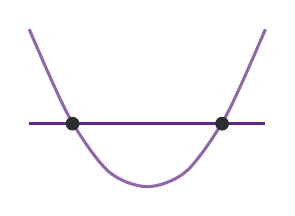
\begin{tikzpicture}
\draw[accent!70,line width=1.1pt] plot [smooth] coordinates {(-15mm,20mm) (-10mm,9mm) (-5mm,2mm) (0,0) (5mm,2mm) (10mm,9mm) (15mm,20mm)};
\draw[accent,line width=1.1pt] (-15mm,8mm) -- (15mm,8mm);
\filldraw[ink] (-9.5mm,8mm) circle (0.8mm);
\filldraw[ink] (9.5mm,8mm) circle (0.8mm);
\end{tikzpicture}
\end{textblock*}

\begin{textblock*}{50mm}(82mm,150mm)
{\centering\fontsize{9.5}{9.5}\selectfont\textbf{Tangent ($D=0$)}\par}
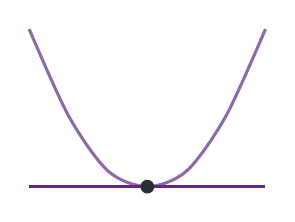
\begin{tikzpicture}
\draw[accent!70,line width=1.1pt] plot [smooth] coordinates {(-15mm,20mm) (-10mm,9mm) (-5mm,2mm) (0,0) (5mm,2mm) (10mm,9mm) (15mm,20mm)};
\draw[accent,line width=1.1pt] (-15mm,0mm) -- (15mm,0mm);
\filldraw[ink] (0,0) circle (0.8mm);
\end{tikzpicture}
\end{textblock*}

\begin{textblock*}{50mm}(138mm,150mm)
{\centering\fontsize{9.5}{9.5}\selectfont\textbf{None ($D<0$)}\par}
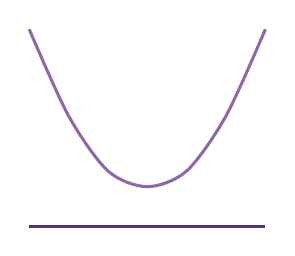
\begin{tikzpicture}
\draw[accent!70,line width=1.1pt] plot [smooth] coordinates {(-15mm,20mm) (-10mm,9mm) (-5mm,2mm) (0,0) (5mm,2mm) (10mm,9mm) (15mm,20mm)};
\draw[accent,line width=1.1pt] (-15mm,-5mm) -- (15mm,-5mm);
\end{tikzpicture}
\end{textblock*}

% ---- CARD 3: Quadratic-quadratic system ----
\cardbg{16}{211}{178}{55}
\pill{26}{214}{Quadratic-quadratic system (kvadrat-kvadrat)}

\begin{textblock*}{158mm}(26mm,227mm)
{\fontsize{11}{14}\selectfont\color{ink}
Same leading coefficient $\to$ subtract the equations to cancel $x^2$,
leaving a linear equation.}
\end{textblock*}

\begin{textblock*}{158mm}(26mm,241mm)
{\fontsize{12}{15}\selectfont
$y=x^2+3x+2,\ y=x^2-x+10\ \Longrightarrow\ 4x=8\ \Longrightarrow\ x=2\ \Longrightarrow\ (2,12)$}
\end{textblock*}

\end{document}
